
%%%%%%%%%%%%%%%%%%%%%%%%%%%%%%%%%%%%%%%%%%%%%%%%%%%%%%%%%%%%%%%%%
%                                                               %
% Chapter: HourglassCorrection Mon Oct 26 18:56:25 EDT 2015
%                                                               %
%%%%%%%%%%%%%%%%%%%%%%%%%%%%%%%%%%%%%%%%%%%%%%%%%%%%%%%%%%%%%%%%%

\chapter{Hourglass Correction}
\label{ch:HourglassCorrection}

\section{Introduction}
As discussed in Chapter ~\ref{ch:SystematicCorrections}, the purpose of
determining $\beta^{*}$ and $\theta_{xing}$ is to correct our luminosity
obtained from the Vernier Scan by using a more realistic model of the beams.
The reason this correction bears the name "Hourglass Correction" is historical
and memetic - the beams when focused in to the IR tend to have the geometry of
an hourglass lying on its side, due to the focusing parameter, $\beta^{*}$,
which would be symmetrical about the nominal $z = 0$ point at the center of the
IR, except for that due to the non-zero crossing crossing angle,
$\theta_{xing}$. This is nomrally not visible, when beams are overlapped at $z =
0$, but when beams are displaced, the characteristic shape can be seen by a
splitting of z-vertex profile. The two humps gain unequal heights when the
crossing angle strays away from zero.

Because the shape of this distriubtion depends on the luminosity integral, we
cannot normally fit the z-vertex profile that we obtain from data. However,
using a Toy Monte-Carlo, we an simulate the z-vertex profile, then compare the
simulated profile using least-squares regression and $\chi^{2}$ comparisons. The
simulation depends on about twenty parameters, which I summarize in
Figure~\ref{fig:sample_configuration}. 

The luminosity of two beams consisting of colloding bunches of any geometry is
described by the convelution of each bunch density over all four space-time
coordinates:

\begin{equation}
  \label{eq:generalluminosity}
  \mathcal{L} = {2 f_{bunch} n_{bunch} N_{blue} N_{yellow} \int \int \int
    \int_{-\infty}^{\infty }\rho^{blue}(x,y,z+ct)\rho^{yellow}(x,y,z-ct)2c\
  dt\ dz\ dx\ dy } 
\end{equation}

\section{Realistically Modeling the Beam}
In simulation, we need to use densities which realistically model the beam's
real shape, ~\cite{herr2006lumi}. We can naievely model the beams in the
transverse direction as simple normal gaussian distriubtions
(Eq~\ref{eq:norm_dist}), assuming head-on collisions
(Figure~\ref{fig:simple_bunch_head_on}).:

\begin{equation}
  \label{eq:norm_dist}
  \rho(x_{i}) = \frac{e^{ -\frac{(x_{i}-\mu)^2}{2\sigma_{x_i}^2}}}{\sigma_{x_i}\sqrt{2\pi}}
\end{equation}

\begin{figure}[ht]
  \begin{center}
    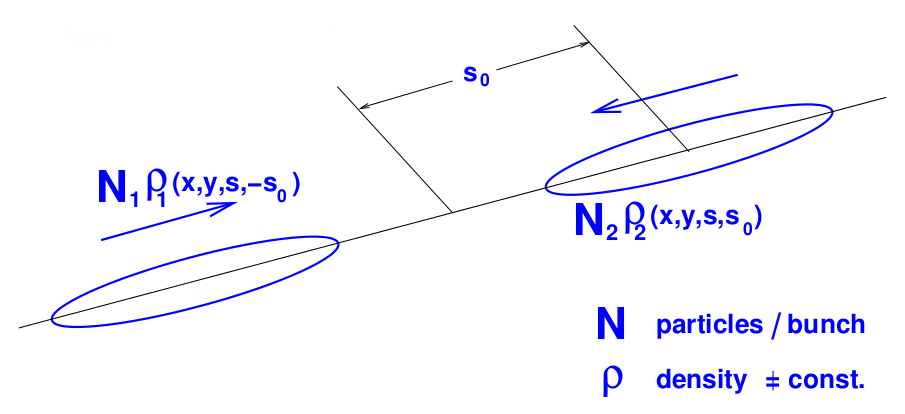
\includegraphics[width=\linewidth,height=\textheight,keepaspectratio]{./figures/simple_bunch_head_on}
    \caption{ 
      Here we see two bunches colliding head on, which is a simplified model
      used to estimate the expected luminsoity, before the application of the
      $\beta^{*}$ squeezing effect and any existence of crossing angles,
      $\theta_{XZ}$ or $\theta_{YZ}$ 
    }
    \label{fig:simple_bunch_head_on}
  \end{center}
\end{figure}

However, equation~\ref{eq:norm_dist} does not capture the true geometry of the
beams. We know that there is a $\beta$ squeeze near the PHENIX IR which squeezes
the beam, focusing it into a smaller area before collissions to boost
luminosity.  We also know that, due the fact that we have intersecting rings,
that there may be some small crossing angle between the bunches. Both of these
effects, $\beta^{*}$ and the crossing angle, affect luminosity. Previous
analyses ~\cite{an888} found the $\beta^{*}$ effect to modify the luminosity by
about 30\%, and the crossing angle by about 1\%.

Recall from Eq~\ref{eq:general_luminosity} that we have four-dimensional
conveluted densities as our integrand for calculation of luminosity. We need to
make some simplifying assumptions about the functional form of these densities,
and then add in corrections to give us a good estimation of beam geometry.
Firstly, we assume that the densities are seperable, i.e.: 

\begin{equation}
  \label{eq:sep_density}
  \rho(x,y,z\pm ct) \rightarrow \rho_{x}(x)\rho_{y}(y)\rho_{z}(z\pm ct)
\end{equation}

We know that the time-dependence of the luminosity is merely to reflect that the
bunches are moving, so there is no "density" in time, from a certain
perspective. We simply observe at the IR two bunches passing through eachother
(sometimes interacting).  This is captured by the $\pm ct$ term in $\rho_{z}$. 

The z-profile of the beams do not have an obvious analytical description.
However, this is not a concern for numerical integration of the luminosity
overlap integral. We can generate these profiles using the wall-current-monitor
data, which also provides a finely binned data stream - giving us sub-nanosecond
resolution on the beam profile in the z-direction. The WCM profile is unique to
a fill, though is constrained to fit into the "beam-buckets" which are simply
areas of low potential containing bunched ions. Angelika Drees from CAD
averaged the profiles for one beam-revolution, and provided them to me. They
are plotted in figures ~\ref{fig:359711_wcm_zprofile},
~\ref{fig:360879_wcm_zprofile}, ~\ref{fig:362492_wcm_zprofile},
~\ref{fig:364636_wcm_zprofile}, ~\ref{fig:365866_wcm_zprofile},
~\ref{fig:366605_wcm_zprofile}, and ~\ref{fig:367138_wcm_zprofile}.

Now, we modify the transverse profiles of tour model in x and y to reflect the
$\beta^{*}$ squeeze, as well as the crossing angles. The $\beta^{*}$ squeeze
will modify the transverse beam widths, introducing a z dependance, so we apply
this trasformation to our simple bunch model. Crossing angles in the XZ and YZ
planes introduce further z-dependance into the x and y bunch distributions, and
additionally introduce x and y dependence into the z-profile. The rotation is
accomplished with a simple coordinate transform.

\begin{equation}
  \label{eq:realistic_transverse_density}
  C_{norm}{e}^{\frac{-{\left(x-\mu_{x}\right)}^2}{2{\left(\sigma\right)}^2}}
\end{equation}

Transformation of the beam widths due to $\beta_{*}$ squeezing (see
Figure~\ref{fig:beta_function}

\begin{gather}
  \label{eq:beta_star_transform}
  \sigma_{i} \rightarrow {{\sigma}_{i}}^{*} =
  \sigma_{i}\sqrt{1+{\left(\frac{z}{\beta^{*}} \right)}^{2} } \\
  i = x, y
\end{gather}


Now apply the rotation, see Figure~\ref{fig:xz_angle}:

\begin{gather}
  \label{eq:transformations}
  x_{blue}   \rightarrow x cos \frac{\phi}{2} - z sin \frac{\phi}{2} \\
  z_{blue}   \rightarrow z cos \frac{\phi}{2} + x sin \frac{\phi}{2} \\
  x_{yellow} \rightarrow x cos \frac{\phi}{2} + z sin \frac{\phi}{2} \\
  z_{yellow} \rightarrow z cos \frac{\phi}{2} - z sin \frac{\phi}{2} \\
  sin \frac {\phi}{2} \rightarrow \frac{\phi}{2} \\
  cos \frac {\phi}{2} \rightarrow 1 + \frac{\phi^2}{4} \\
  x_{blue}^{R}  = x\left(1+\frac{{\phi}^{2}}{4}\right)- z \frac{\phi}{2} \\
  z_{blue}^{R}  = z\left(1+\frac{{\phi}^{2}}{4}\right)+ x \frac{\phi}{2} \\
  x_{yellow}^{R}= x\left(1+\frac{{\phi}^{2}}{4}\right)+ z \frac{\phi}{2} \\
  z_{yellow}^{R}= z\left(1+\frac{{\phi}^{2}}{4}\right)- z \frac{\phi}{2} \\
\end{gather}

Rather then write down the final (frankly hideous) form of the luminsoity
integral, I will instead write it down in terms of these transformed
coordinates.

\begin{gather}
  \label{eq:final_luminosity}
  {{\sigma}_{i}}^{*} \rightarrow \sigma_{i}^{*R} =
  \sigma_{i}\sqrt{1+{\left(\frac{z^{R}}{\beta^{*}} \right)}^{2} } \\
  \rho_{x_i}(x_{i}) \rightarrow \rho_{x_{i}^{R}}^{*}(x_{i}^{R}) = C_{x_{i}}{e}^{\frac{-{\left(x_{i}^{R}-\mu_{x}\right)}^2}{2{\left(\sigma_{i}^{*R}\right)}^2}} \\
  i = x,y \\
\end{gather}

We plug the separable models for density into the luminosity integral to obtain
our final form. Although the simple gaussian integration can be normalized
ahead of time due to knowlege of that function's total integral, in this case,
it may be neccessary to numerically integrate the density functions, and apply
an overall normalization.

\clearpage
\begin{figure}[ht]
  \centering
  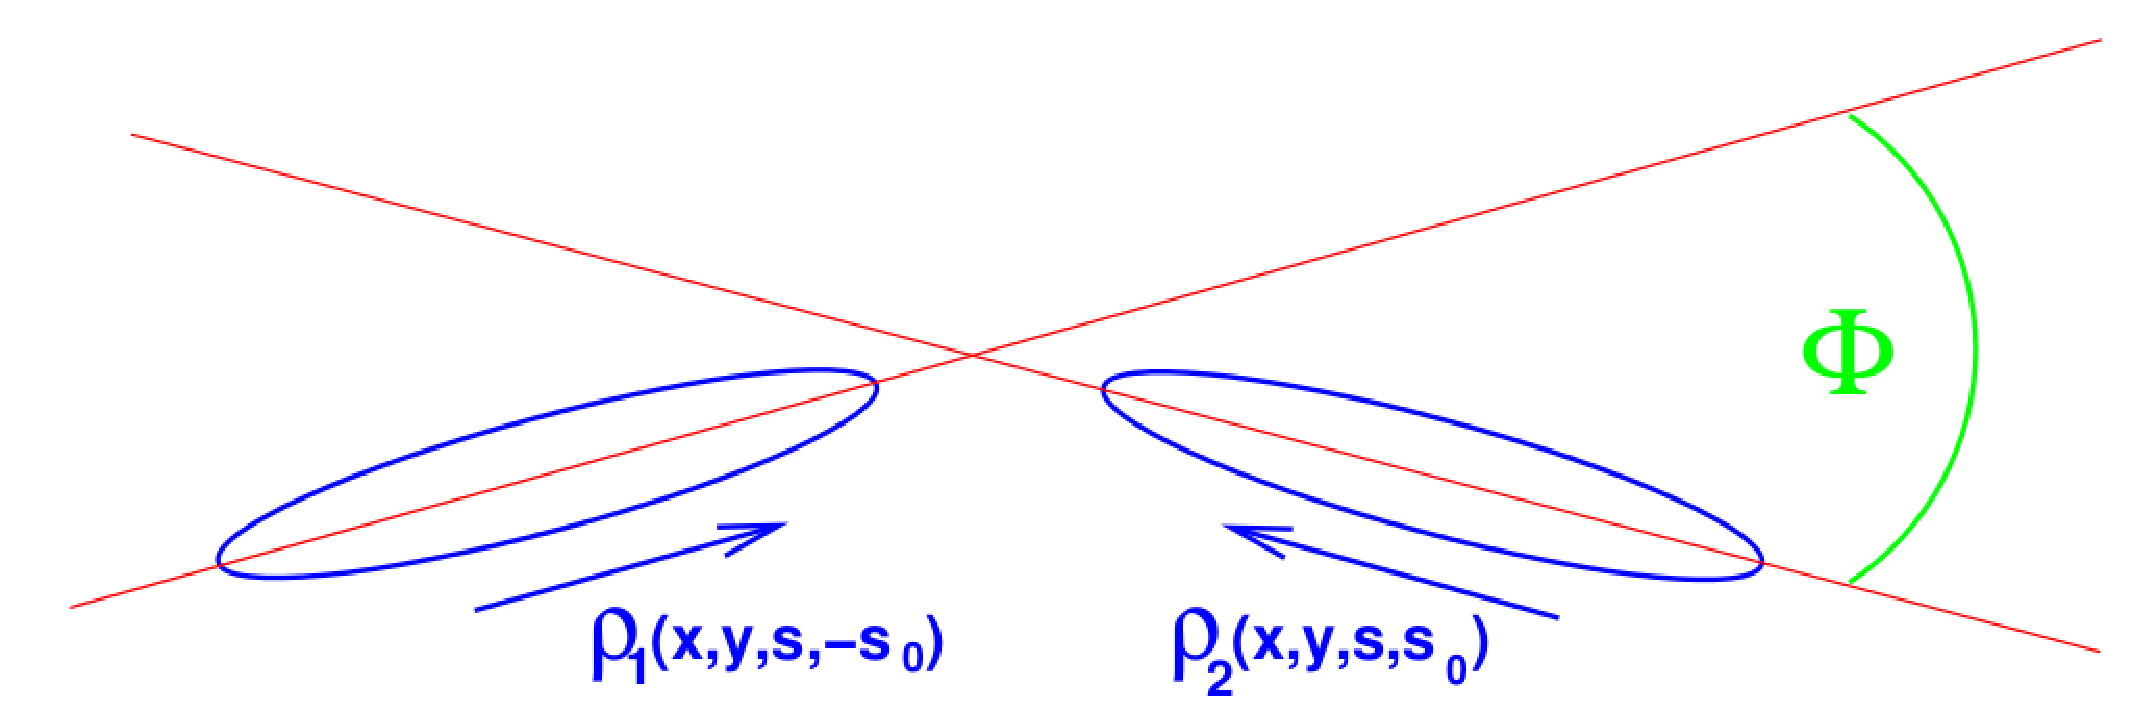
\includegraphics[width=\linewidth,height=0.5\textheight,keepaspectratio]{./figures/xing_bunch}
  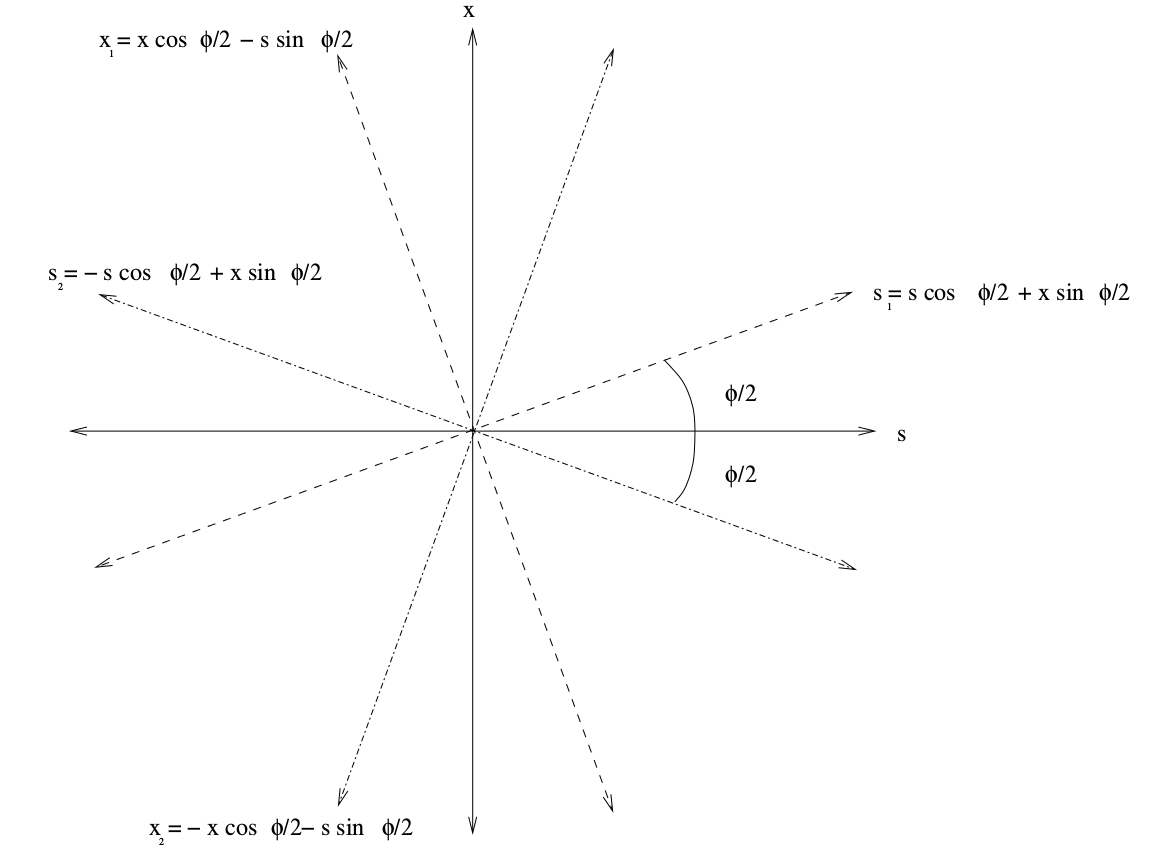
\includegraphics[width=\linewidth,height=0.5\textheight,keepaspectratio]{./figures/bunch_rotation}
  \caption{ 
    Here, we see a schematic view of the coordinate rotation due to the crossing
    angle (in this case we see the XZ plane, but the situation is identical in the
    YZ plane).
  }
  \label{fig:xz_angle}
\end{figure}


\begin{figure}
  \centering
  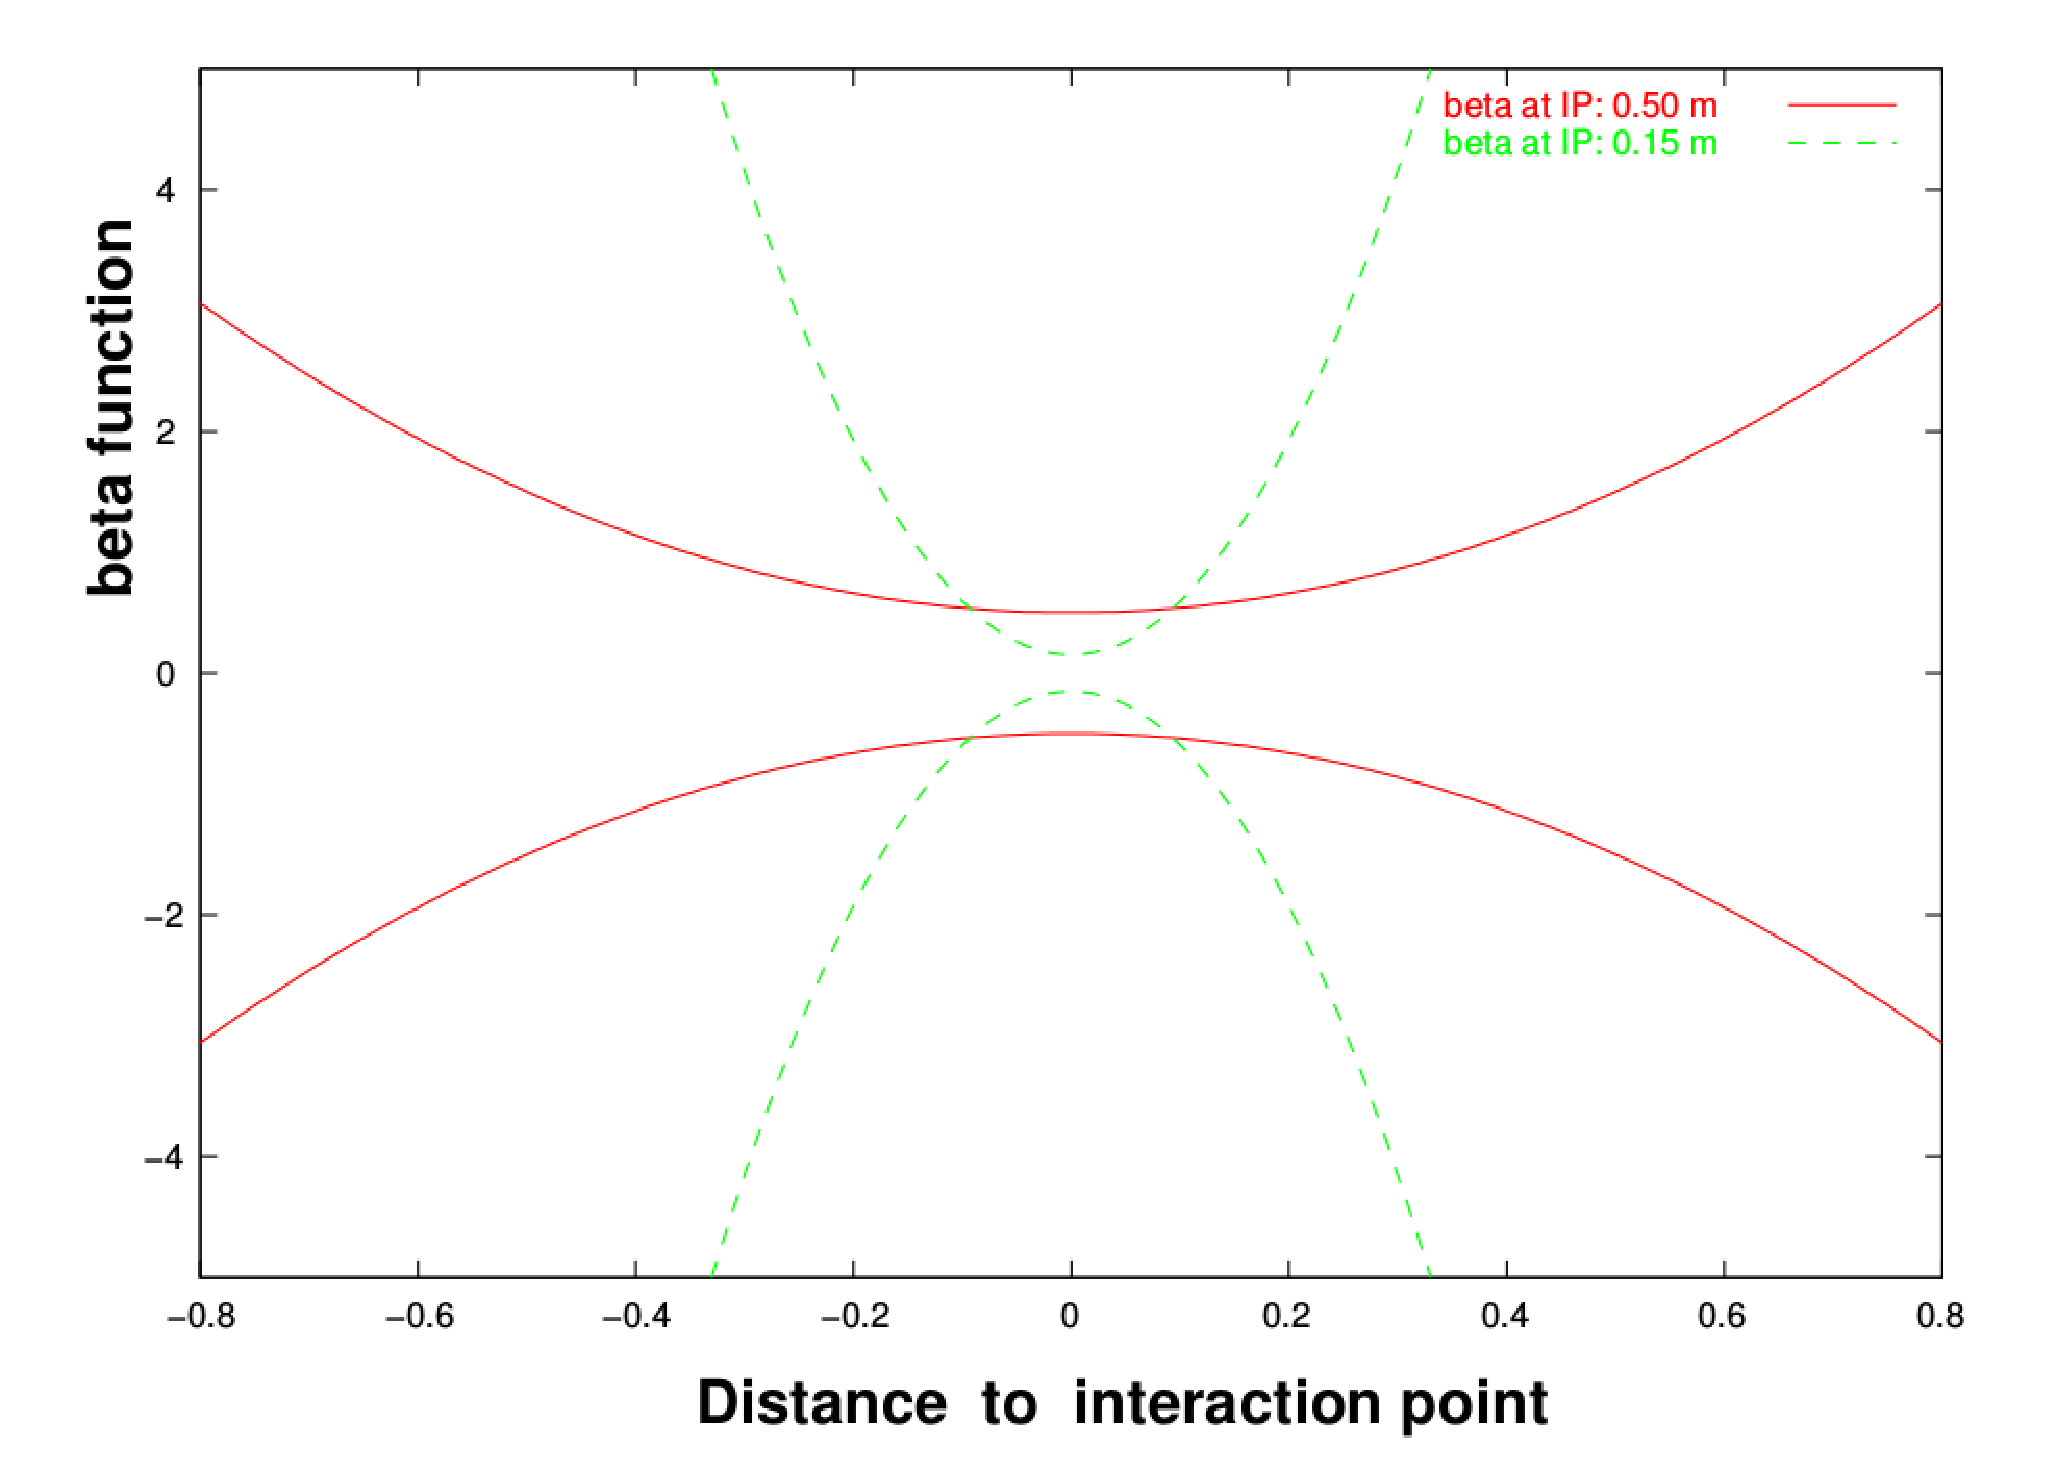
\includegraphics[width=\linewidth,height=\textheight,keepaspectratio]{./figures/beta_function}
  \caption{
    Here, we see a function of z, $\beta^{*}$, which shows the shape of the
    squeezing potential in one of the planes. Two different values of
    $\beta^{*}$ are shown.
  }
  \label{fig:beta_function}
\end{figure}
\clearpage

\begin{figure}[ht]
  \centering
  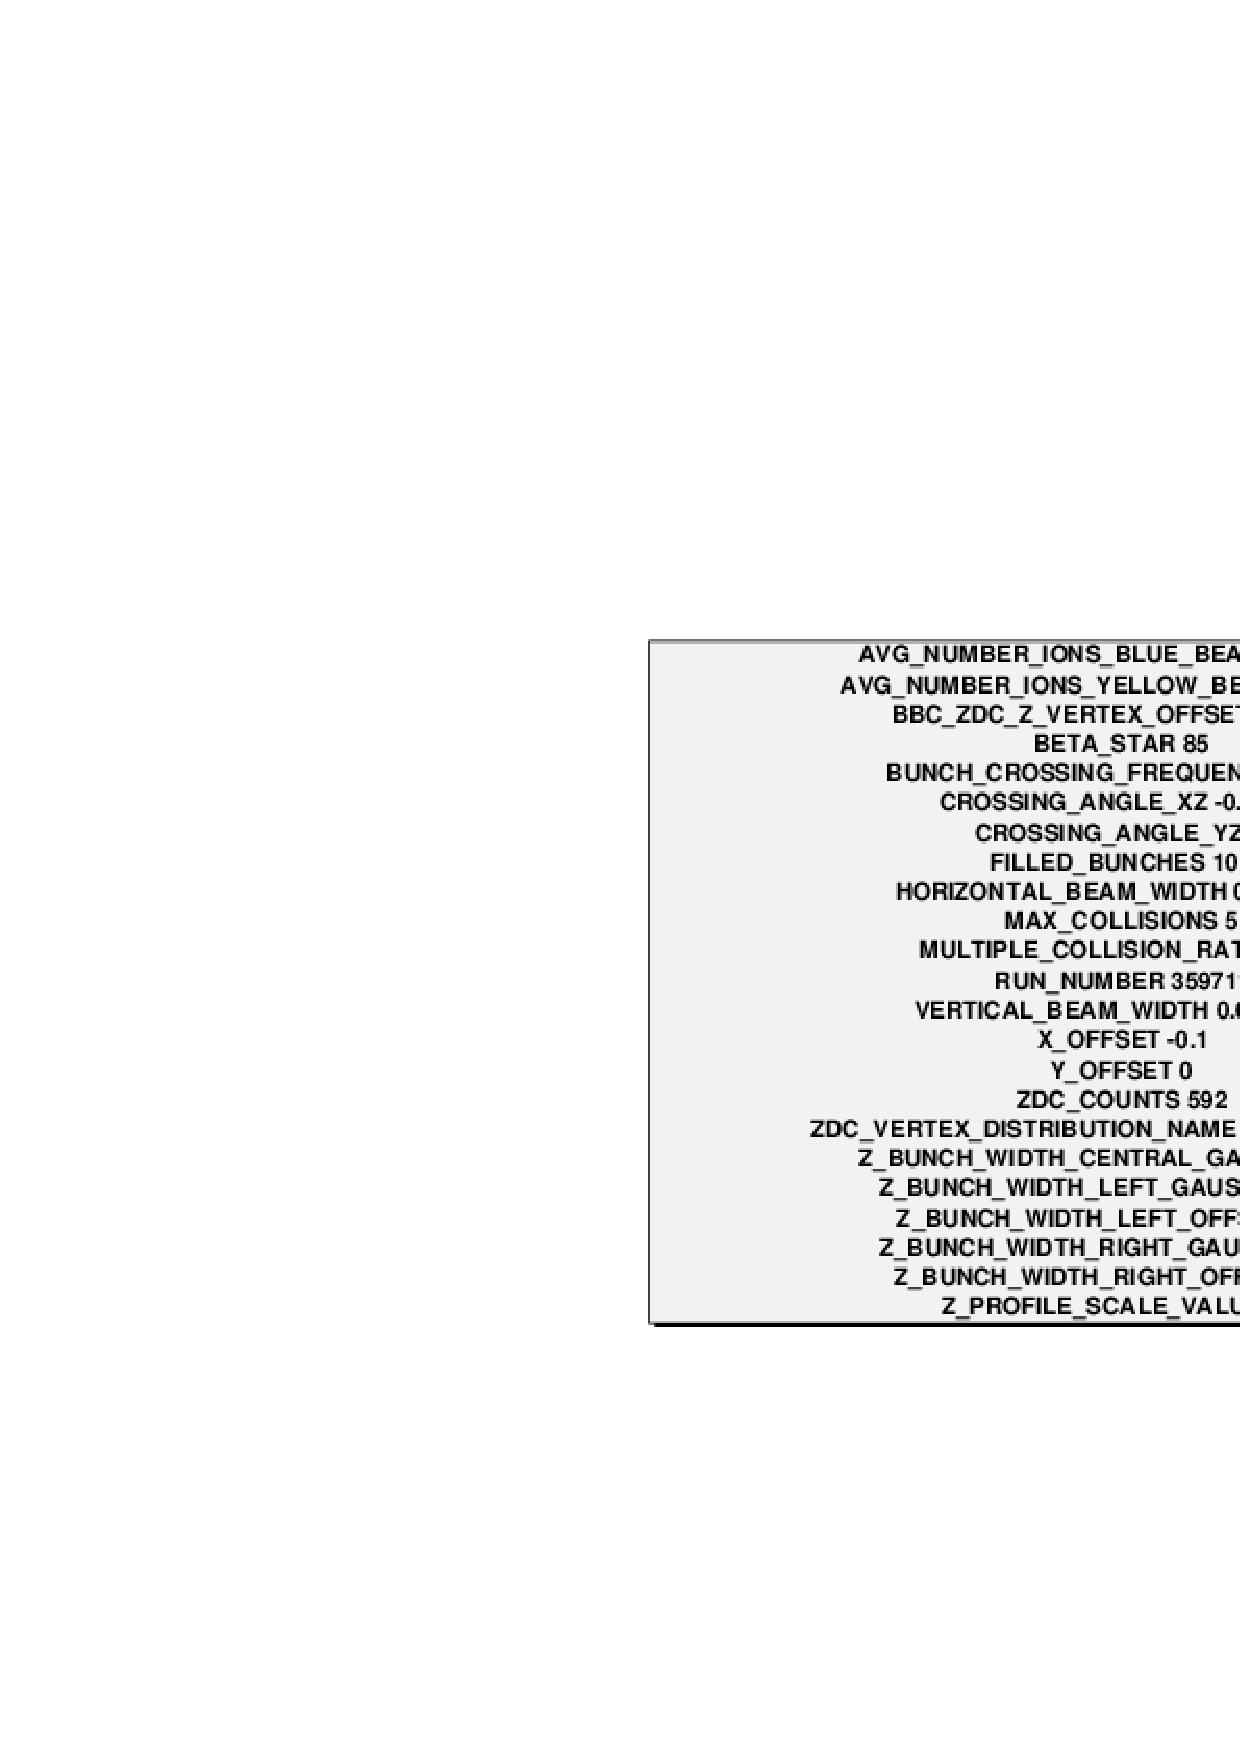
\includegraphics[width=\linewidth,height=\textheight,keepaspectratio]{./figures/sample_configuration}
  \caption{
    Each parameter is initialized directly from data. Parameters which are our
    goal to determine, $\beta^{*}$ and $\theta_{xing}$ are obtained from
    reasonable ranges predicted by CAD, and then varied until good agreement is
    reached.
  }
  \label{fig:sample_configuration}
\end{figure}

\section{Monte Carlo Simulation and Numerically Integrated Luminosity}
The toy Monte Carlo is seeded with initial values which are extracted from the
data, and then the parameters are adjusted until suitably matching the data
distribution.

Within the toy Monte-Carlo, we calculate the full form of the Luminosity, by
making a few simplifying assumptions.

\begin{itemize}
  \item All bunches are identical
  \item Beam widths obtained from the vernier scan are good approximations
  \item Which bunches are filled/unfilled do not matter, so long as we have the
    correct number of filled bunches.
  \item There is no crossing angle in the z-y plane, only the z-x plane (this
    can be verified as a good assumption by observing figure (FIGURE
    REFERENCE NEEDED)
\end{itemize}

Once we simulate the luminosity, we compare this to the overall luminosity
obtained directly from the data (but without correction for the hourglass effect
or crossing angle). We obtain the ratio of the two luminosities, thus yielding
our multiplicative correction factor.

Within the simulation, we calculate the luminosity via a riemann sum, binning
space and time finely enough to converge to a reasonable value.

The general work flow of the simulation and minimization process is modeled
schematically in ~\ref{fig:simulation_flow}. 

\begin{figure}[ht]
\begin{center}
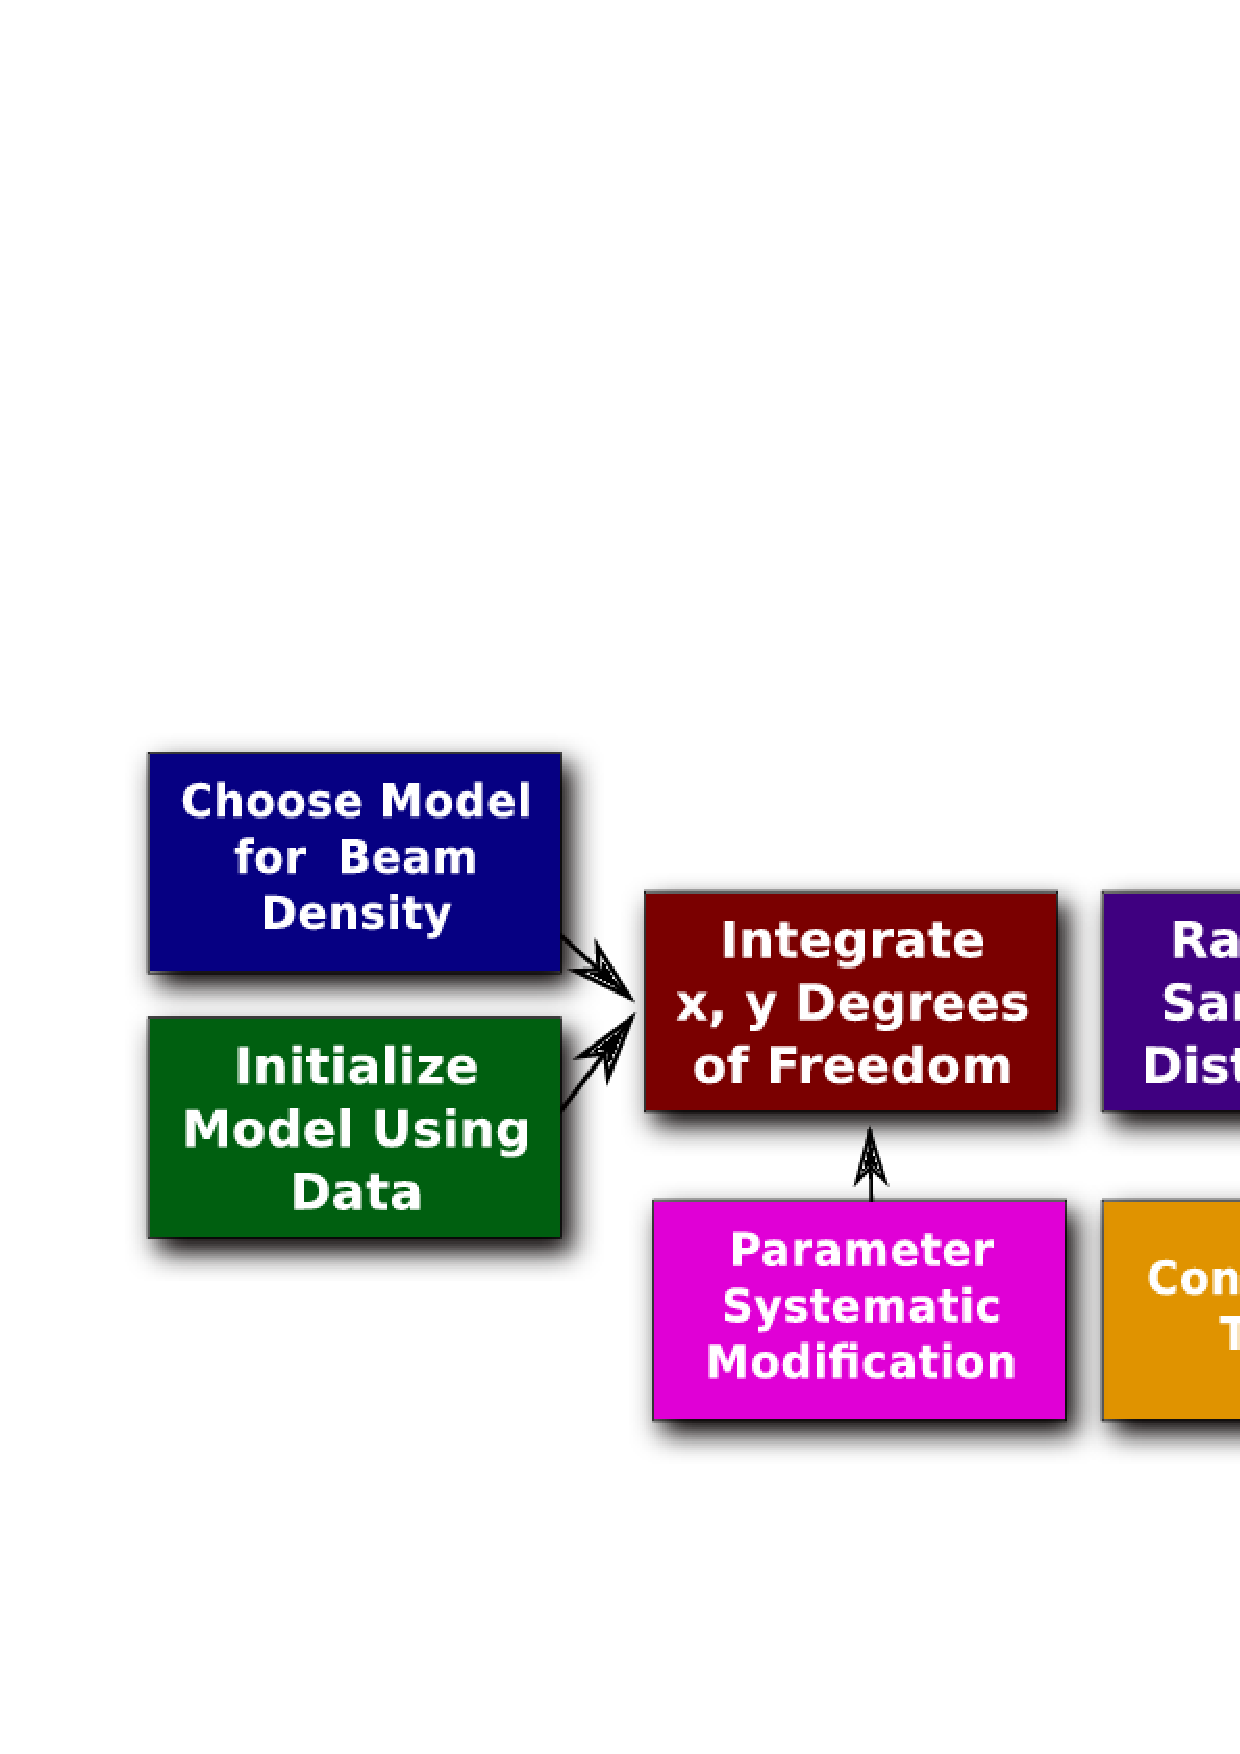
\includegraphics[width=\linewidth,height=\textheight,keepaspectratio]{./figures/simulation_flow}
\caption{
Here we see the schematic overview of the simulation. Each box represents a
distinct step we take in the modeling or numeric integration of the luminosity.
Because we use numeric methods for solving the luminosity integral, we do not
have easy access to regression methods such as gradient-descent. Instead we
start matching the zdc z-vertex profile with the simulated profile, and then
vary the configuration parameters over reasonable ranges, choosing the result
which minimizes the difference between the distributions.
}
\label{fig:simulation_flow}
\end{center}
\end{figure}
\clearpage

\begin{figure}
\begin{center}
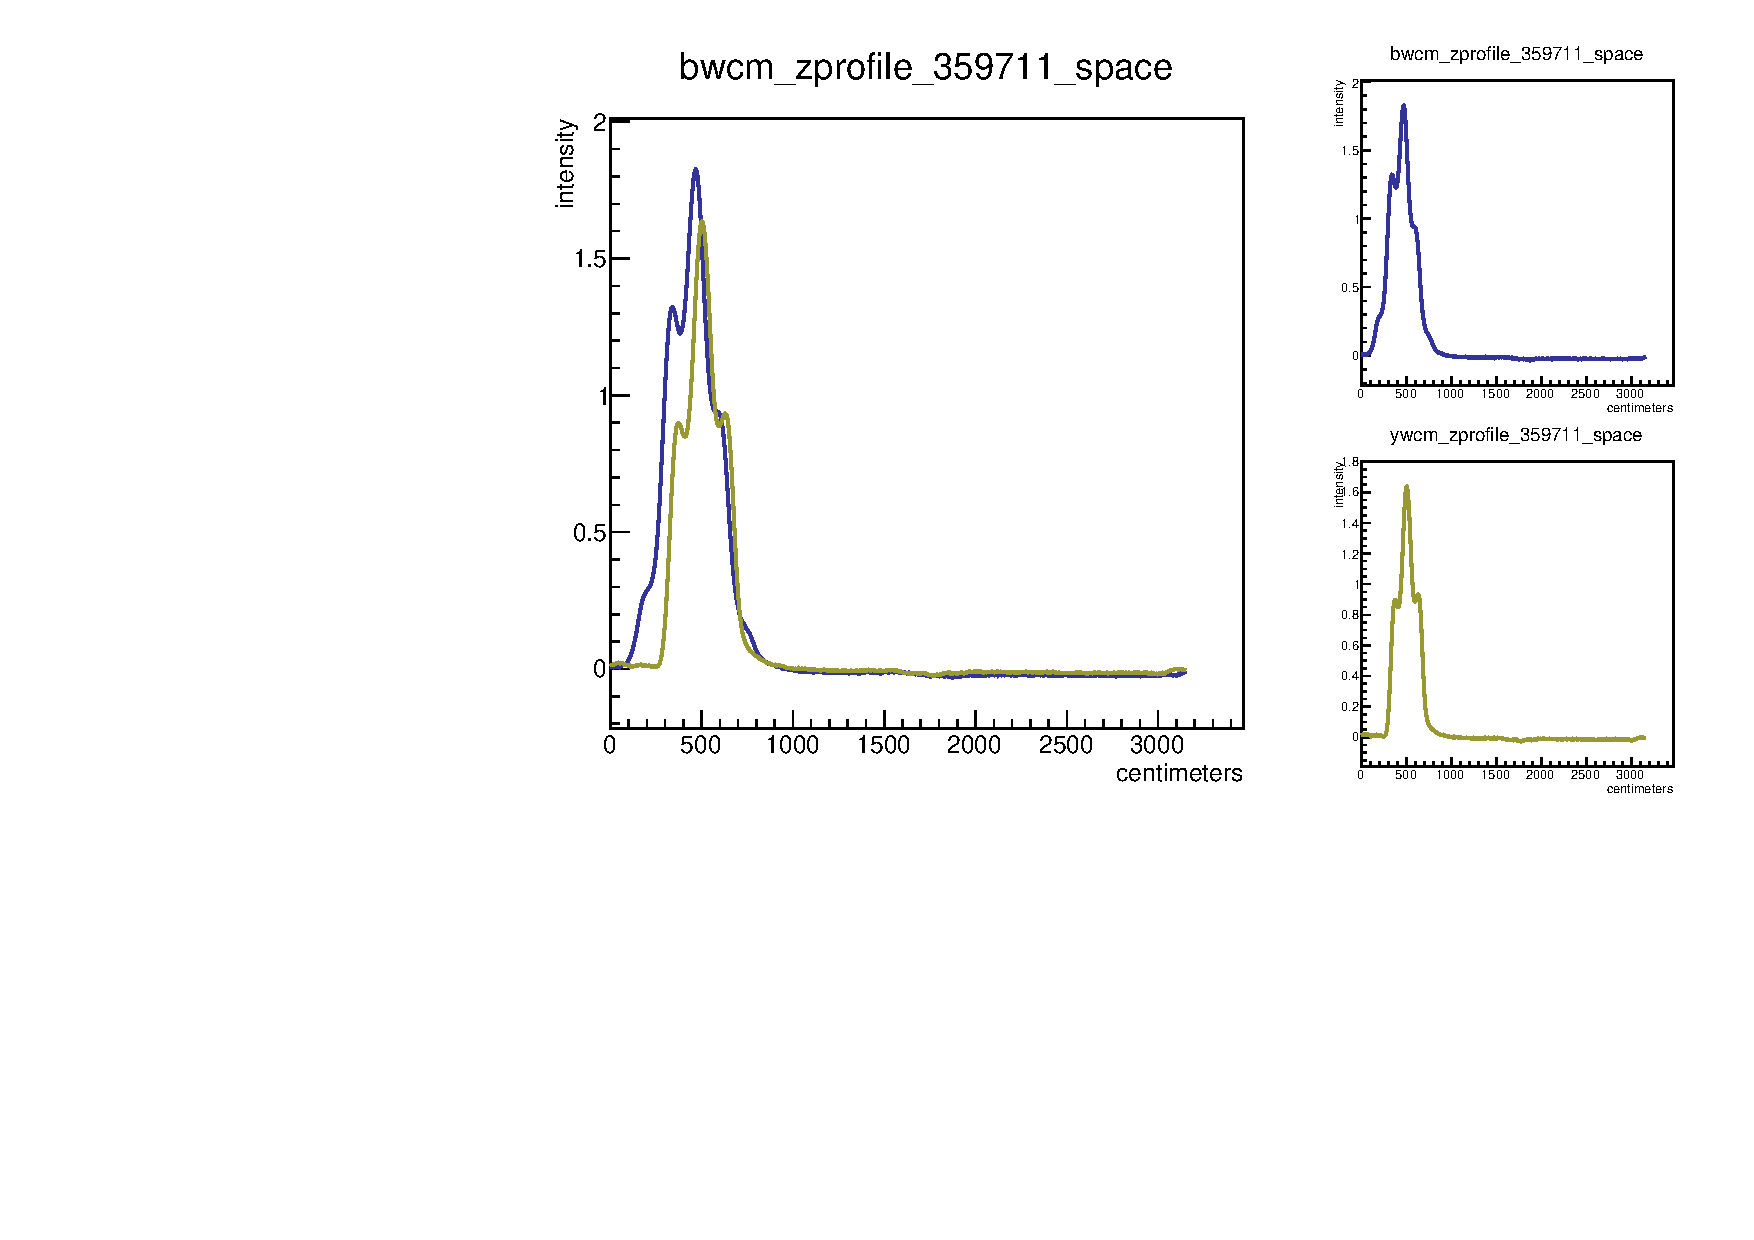
\includegraphics[width=\linewidth,height=\textheight,keepaspectratio]{./figures/359711_wcm_zprofile}
\caption{ 
Left: the blue and yellow wall current monitor beam z-profiles. One can see the
three beam buckets which make up one so-called "filled bunch". Bunches are
approximately 1000 cm long, the entire profile passes the IR once every 106
nanoseconds, though most of the bunch is actually within a time envelope of
approximately 35 nanosecons. The panes on the right show the blue beam (top)
and the yellow beam (bottom).
}
\label{fig:359711_wcm_zprofile}
\end{center}
\end{figure}

\begin{figure}
\begin{center}
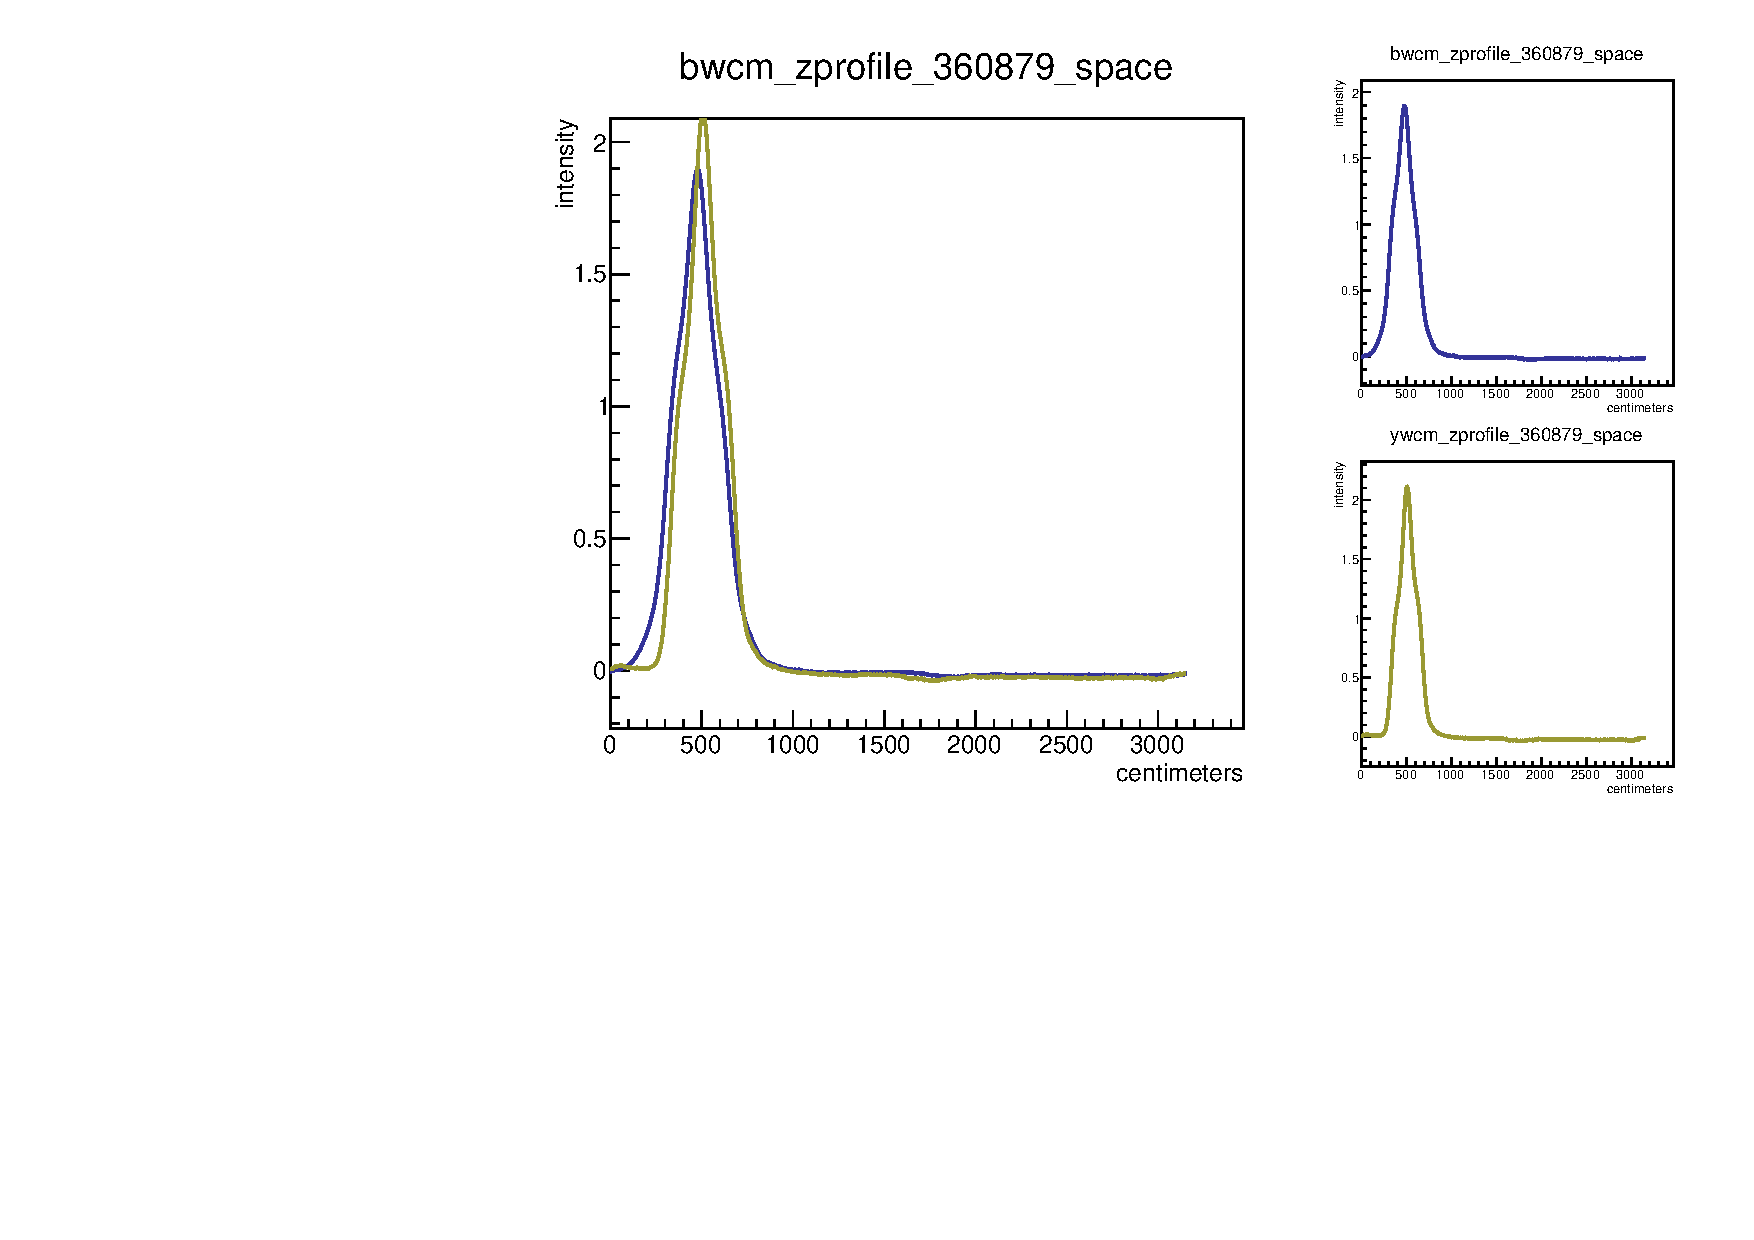
\includegraphics[width=\linewidth,height=\textheight,keepaspectratio]{./figures/360879_wcm_zprofile}
\caption{ 
Left: the blue and yellow wall current monitor beam z-profiles. One can see the
three beam buckets which make up one so-called "filled bunch". Bunches are
approximately 1000 cm long, the entire profile passes the IR once every 106
nanoseconds, though most of the bunch is actually within a time envelope of
approximately 35 nanosecons. The panes on the right show the blue beam (top)
and the yellow beam (bottom).
}
\label{fig:360879_wcm_zprofile}
\end{center}
\end{figure}


\begin{figure}
\begin{center}
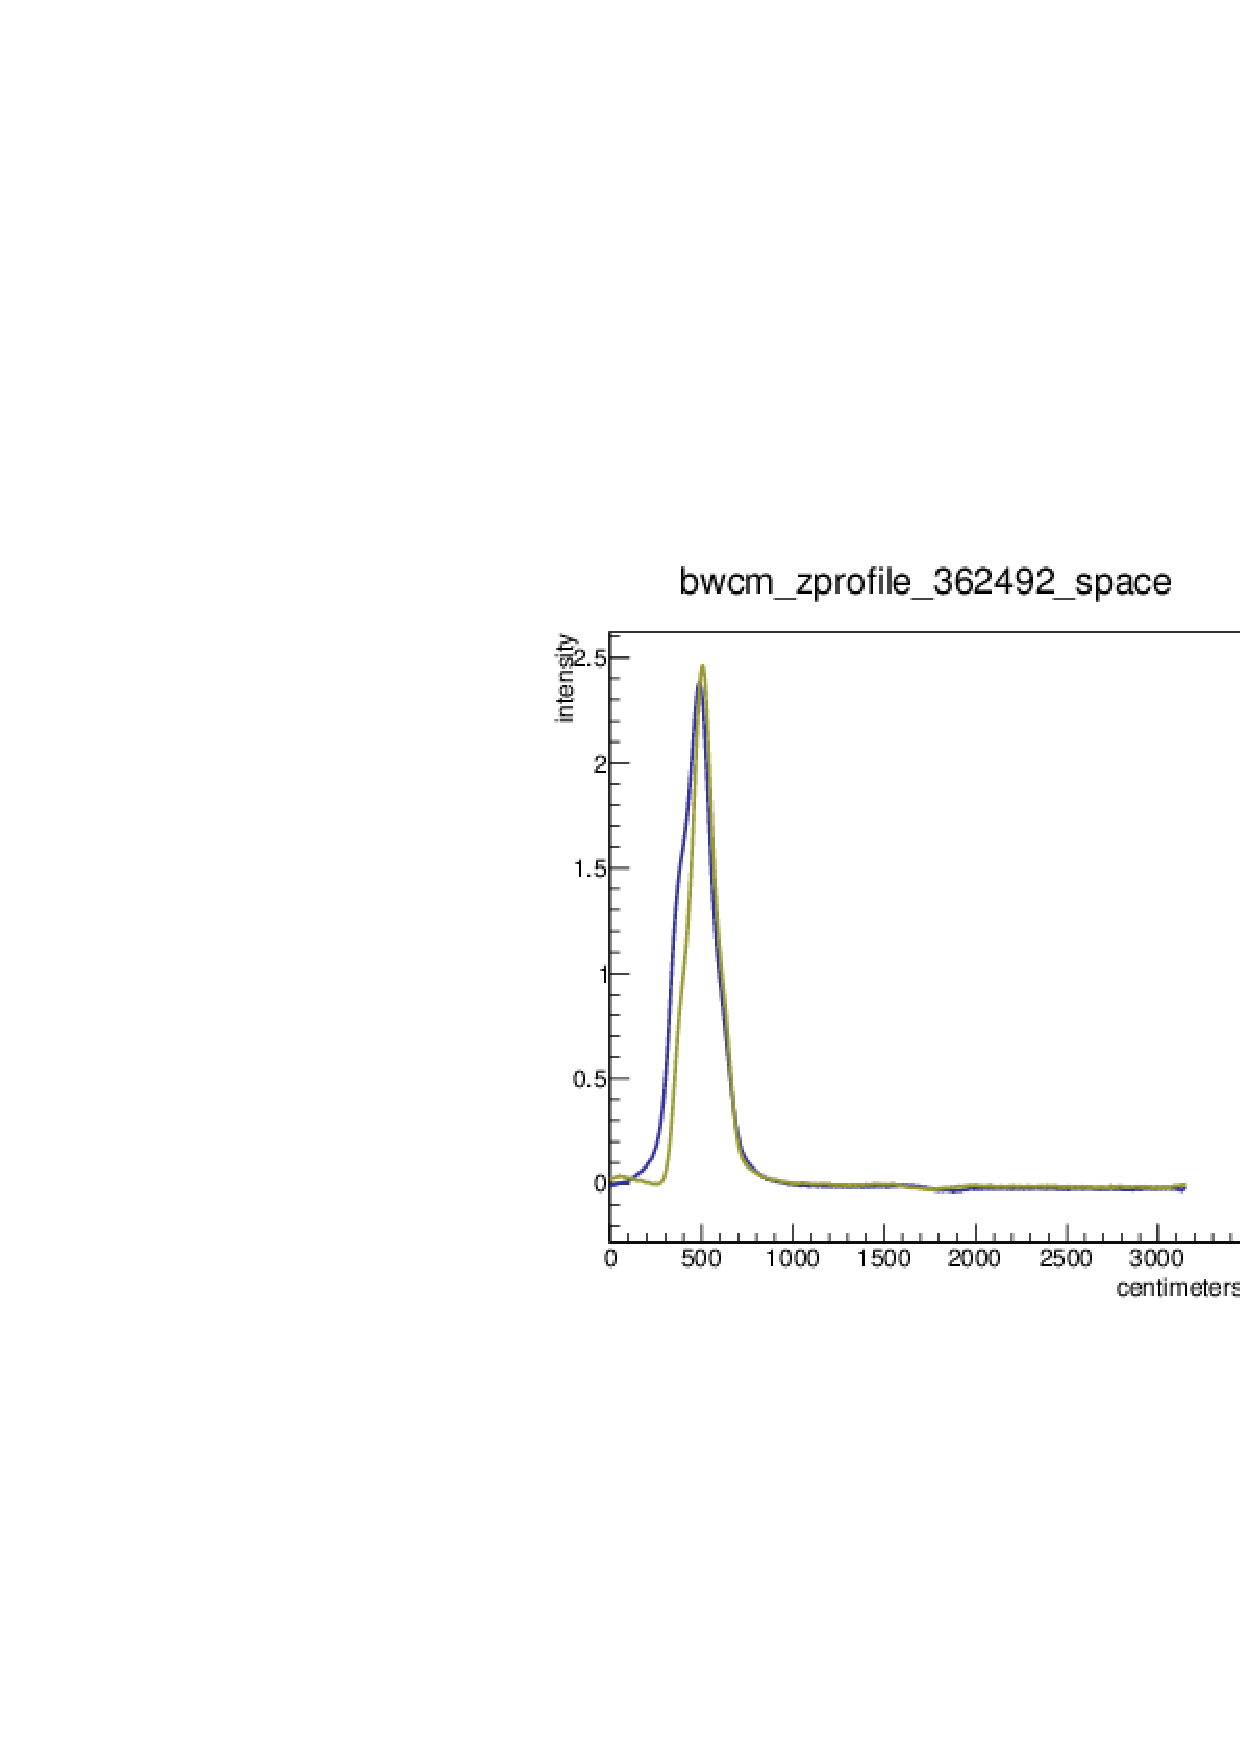
\includegraphics[width=\linewidth,height=\textheight,keepaspectratio]{./figures/362492_wcm_zprofile}
\caption{ 
Left: the blue and yellow wall current monitor beam z-profiles. One can see the
three beam buckets which make up one so-called "filled bunch". Bunches are
approximately 1000 cm long, the entire profile passes the IR once every 106
nanoseconds, though most of the bunch is actually within a time envelope of
approximately 35 nanosecons. The panes on the right show the blue beam (top)
and the yellow beam (bottom).
}
\label{fig:362492_wcm_zprofile}
\end{center}
\end{figure}

\begin{figure}
\begin{center}
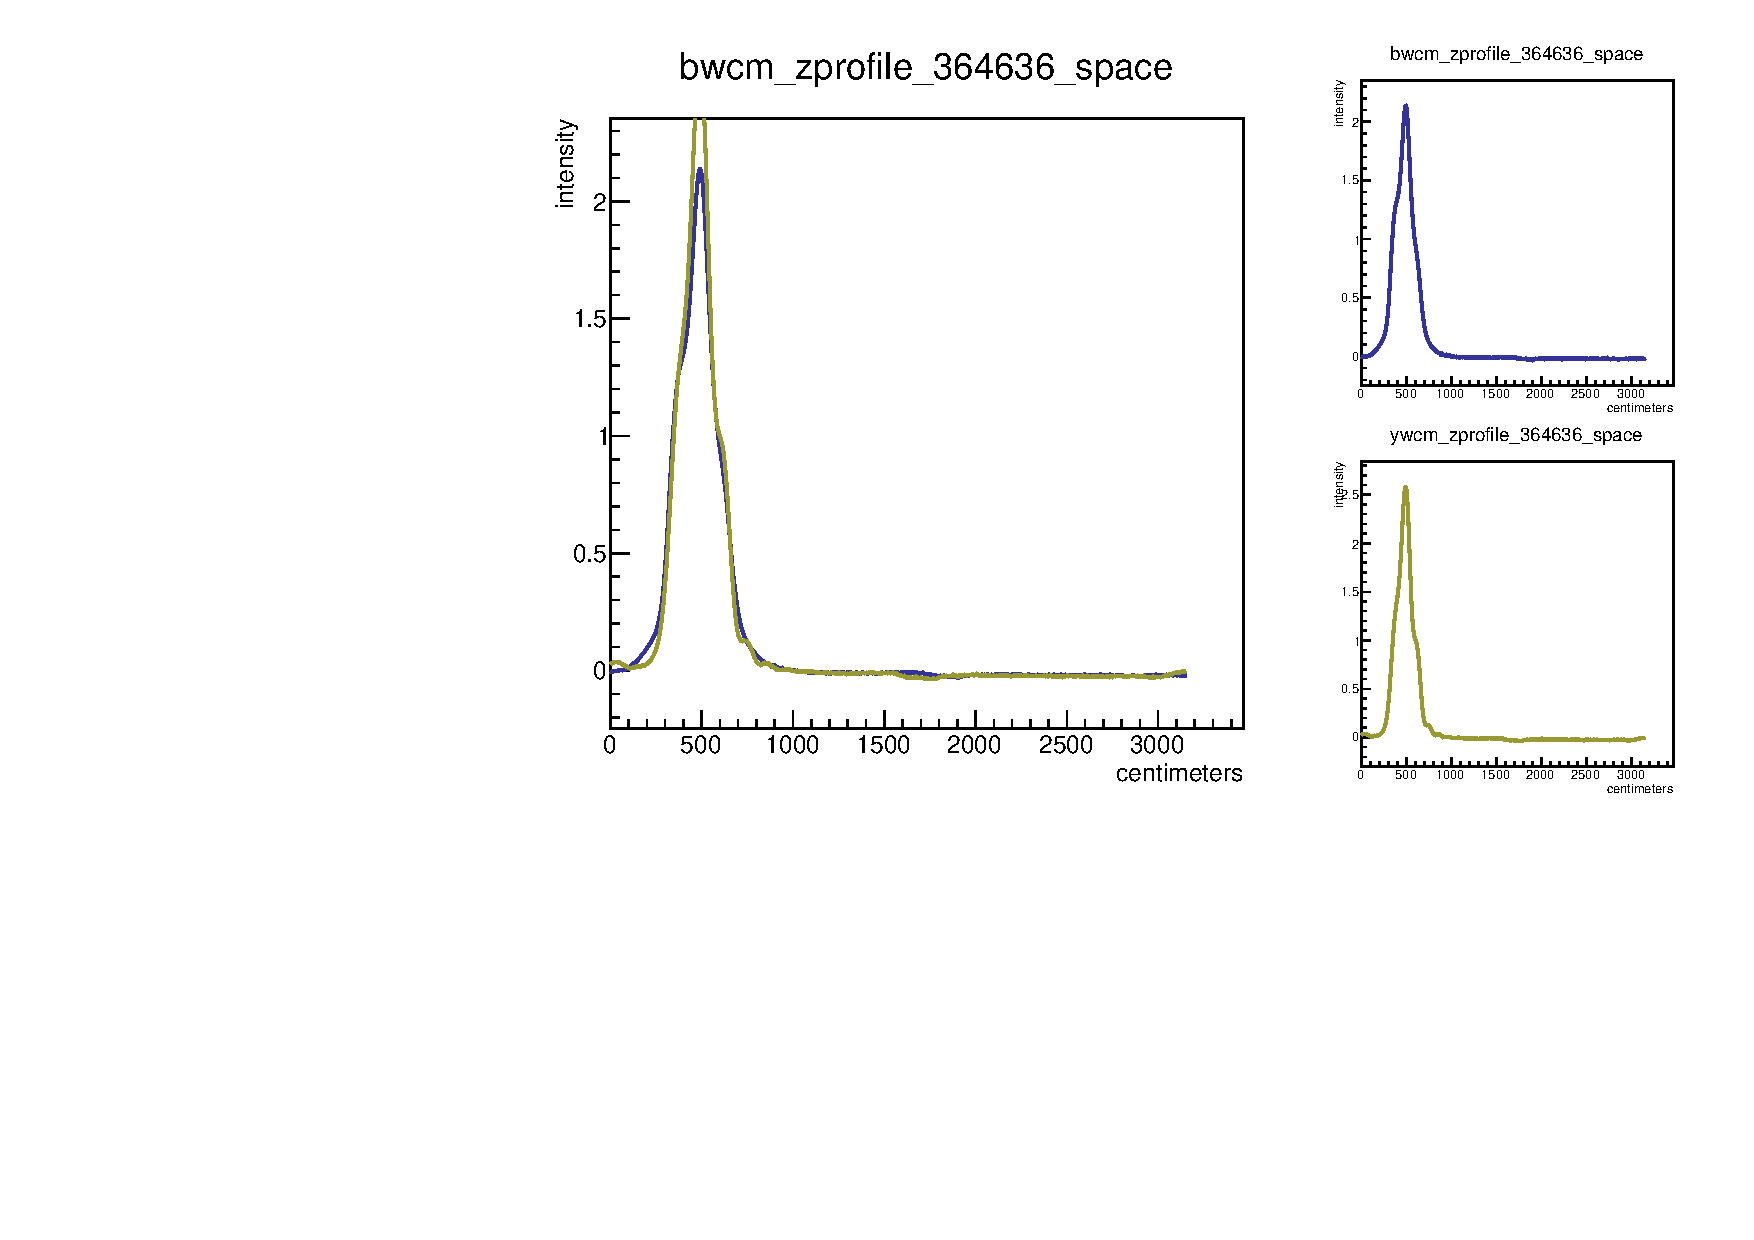
\includegraphics[width=\linewidth,height=\textheight,keepaspectratio]{./figures/364636_wcm_zprofile}
\caption{ 
Left: the blue and yellow wall current monitor beam z-profiles. One can see the
three beam buckets which make up one so-called "filled bunch". Bunches are
approximately 1000 cm long, the entire profile passes the IR once every 106
nanoseconds, though most of the bunch is actually within a time envelope of
approximately 35 nanosecons. The panes on the right show the blue beam (top)
and the yellow beam (bottom).
}
\label{fig:364636_wcm_zprofile}
\end{center}
\end{figure}

\begin{figure}
\begin{center}
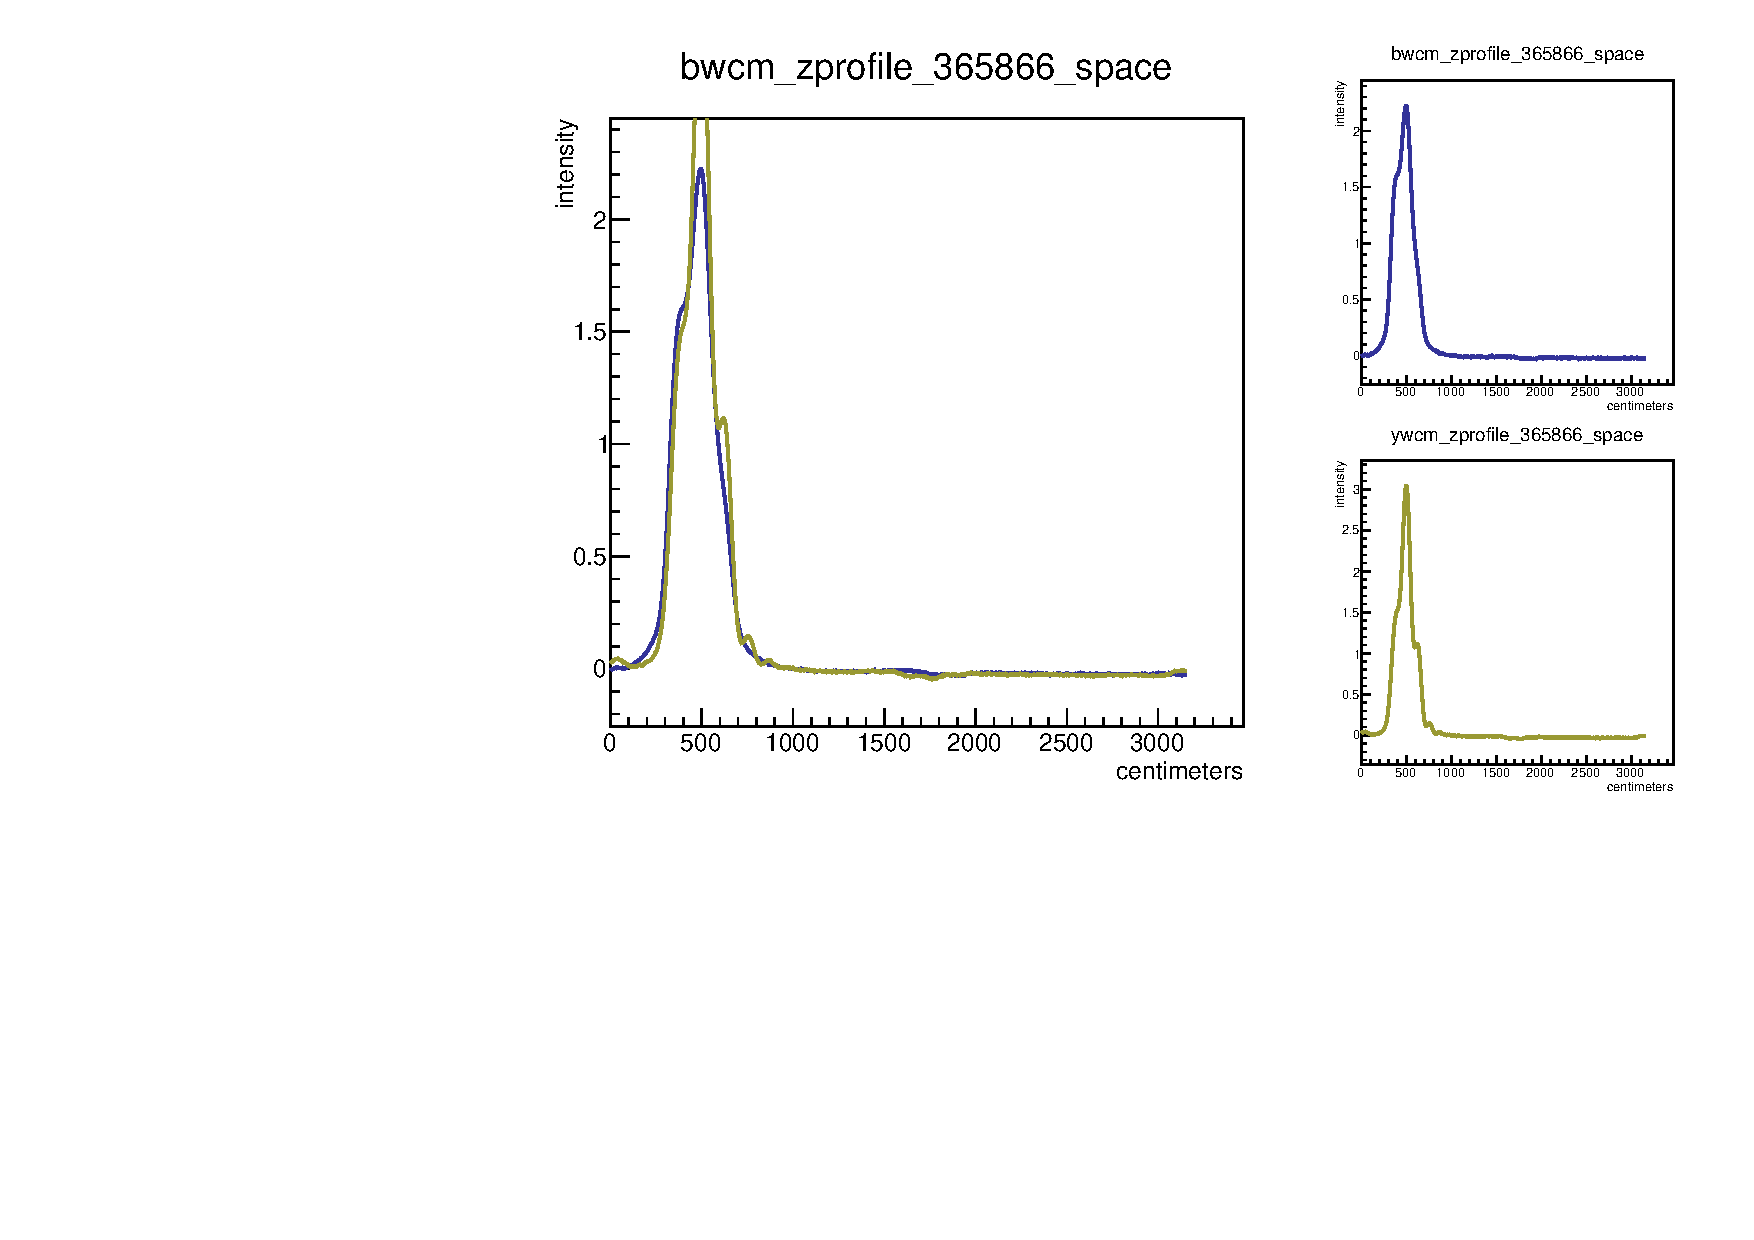
\includegraphics[width=\linewidth,height=\textheight,keepaspectratio]{./figures/365866_wcm_zprofile}
\caption{ 
Left: the blue and yellow wall current monitor beam z-profiles. One can see the
three beam buckets which make up one so-called "filled bunch". Bunches are
approximately 1000 cm long, the entire profile passes the IR once every 106
nanoseconds, though most of the bunch is actually within a time envelope of
approximately 35 nanosecons. The panes on the right show the blue beam (top)
and the yellow beam (bottom).
}
\label{fig:365866_wcm_zprofile}
\end{center}
\end{figure}

\begin{figure}
\begin{center}
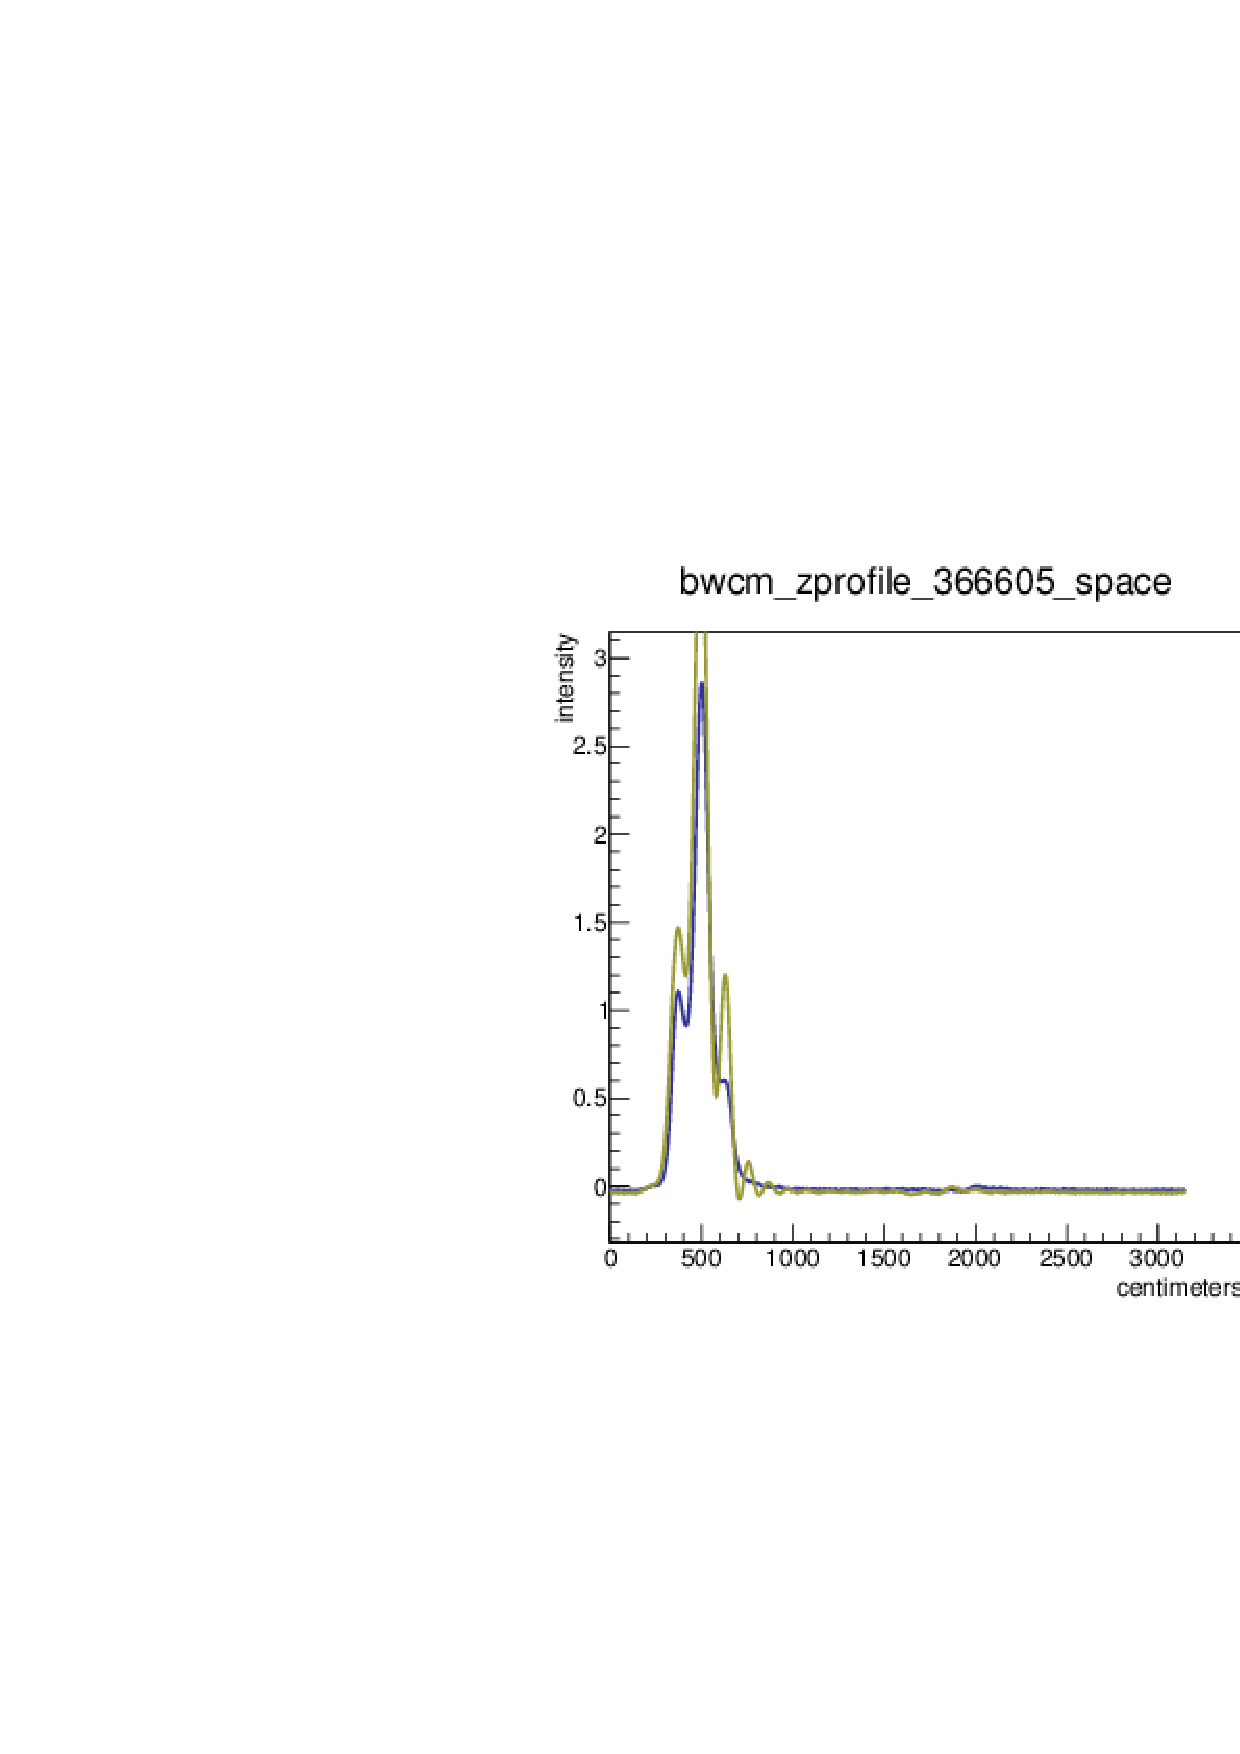
\includegraphics[width=\linewidth,height=\textheight,keepaspectratio]{./figures/366605_wcm_zprofile}
\caption{ 
Left: the blue and yellow wall current monitor beam z-profiles. One can see the
three beam buckets which make up one so-called "filled bunch". Bunches are
approximately 1000 cm long, the entire profile passes the IR once every 106
nanoseconds, though most of the bunch is actually within a time envelope of
approximately 35 nanosecons. The panes on the right show the blue beam (top)
and the yellow beam (bottom).
}
\label{fig:366605_wcm_zprofile}
\end{center}
\end{figure}

\begin{figure}
\begin{center}
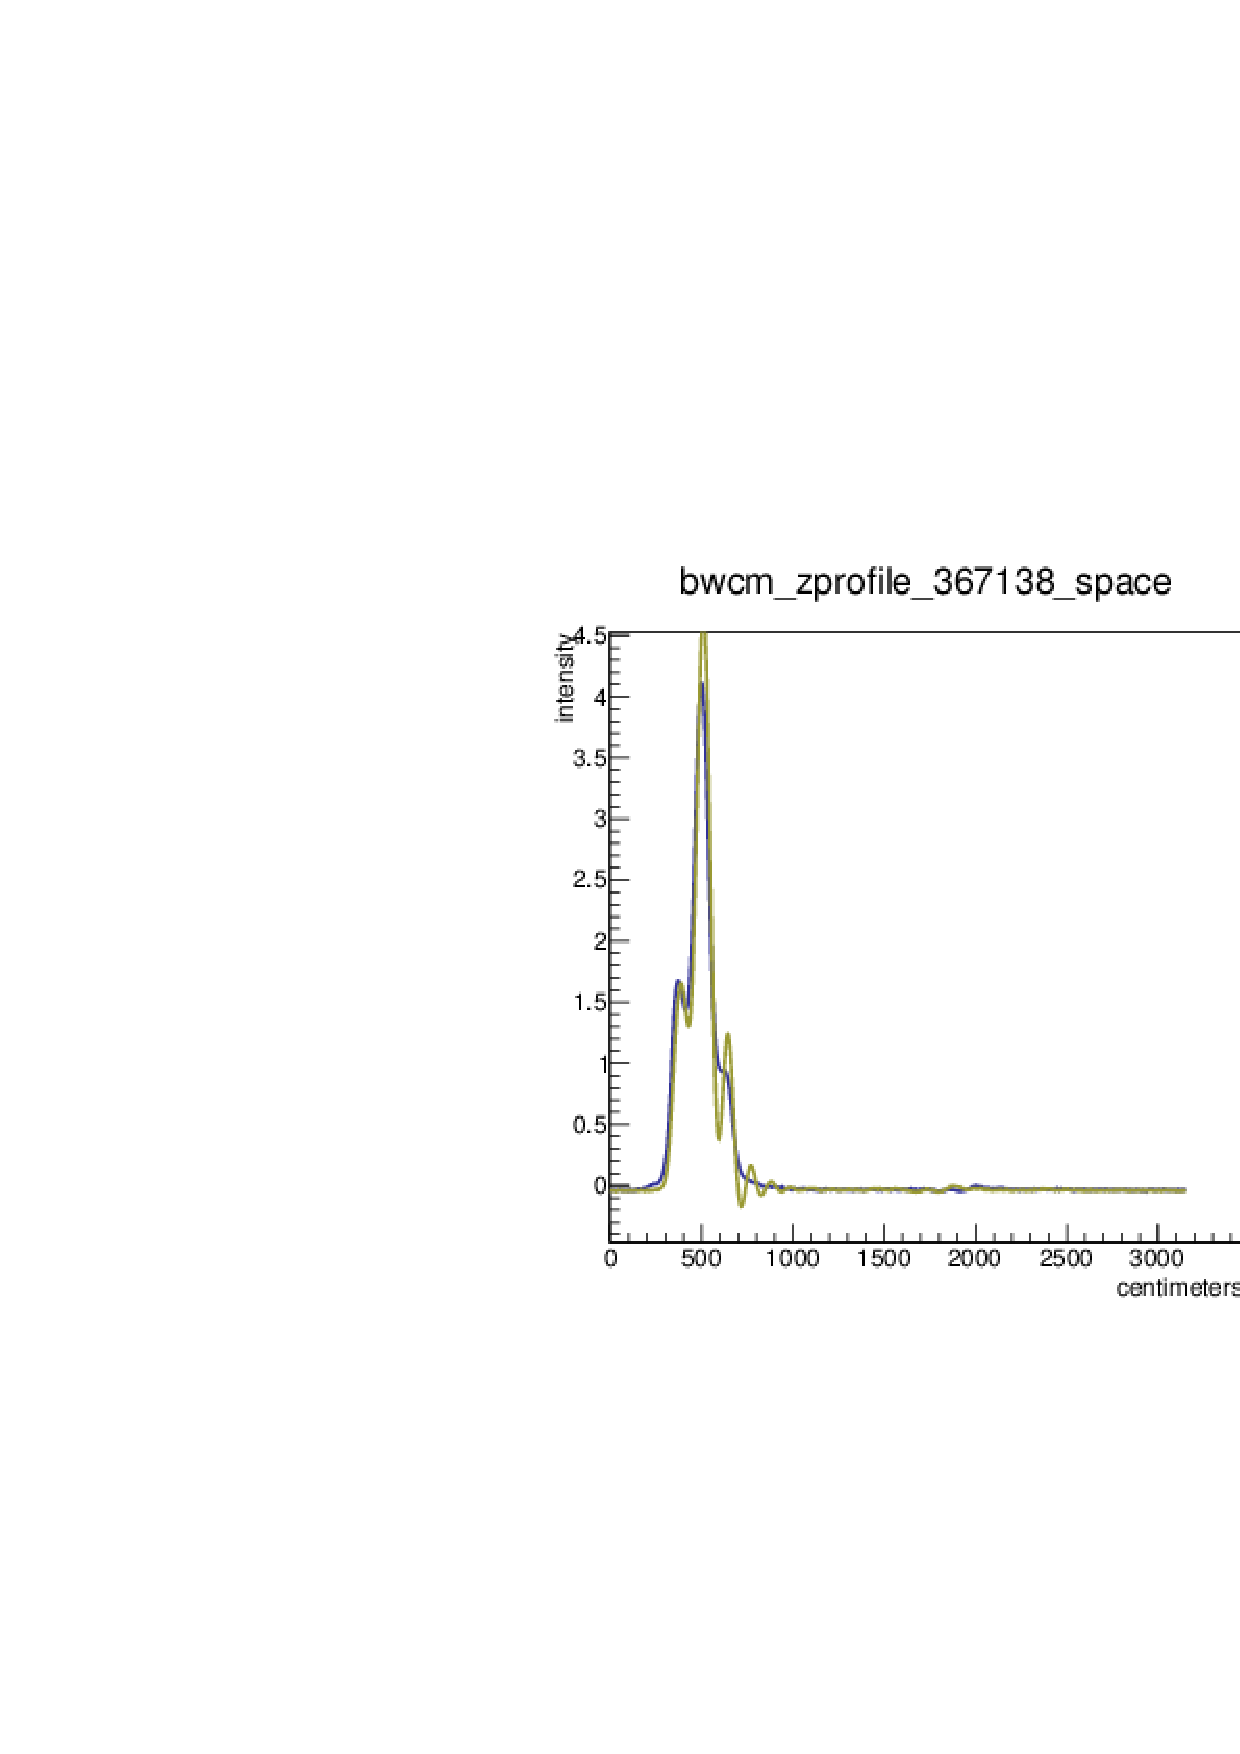
\includegraphics[width=\linewidth,height=\textheight,keepaspectratio]{./figures/367138_wcm_zprofile}
\caption{ 
Left: the blue and yellow wall current monitor beam z-profiles. One can see the
three beam buckets which make up one so-called "filled bunch". Bunches are
approximately 1000 cm long, the entire profile passes the IR once every 106
nanoseconds, though most of the bunch is actually within a time envelope of
approximately 35 nanosecons. The panes on the right show the blue beam (top)
and the yellow beam (bottom).
}
\label{fig:367138_wcm_zprofile}
\end{center}
\end{figure}
\clearpage

\subsection{Hourglass Simulation Parameter Space}

I systematically explored the hourglass parameter space to try and determine the
best set of intial parameters to use to configure the starting point for the
brute force regression. An example is seen in
Figure~\ref{359711_step14_config_compare}. 

\begin{figure}
\begin{center}
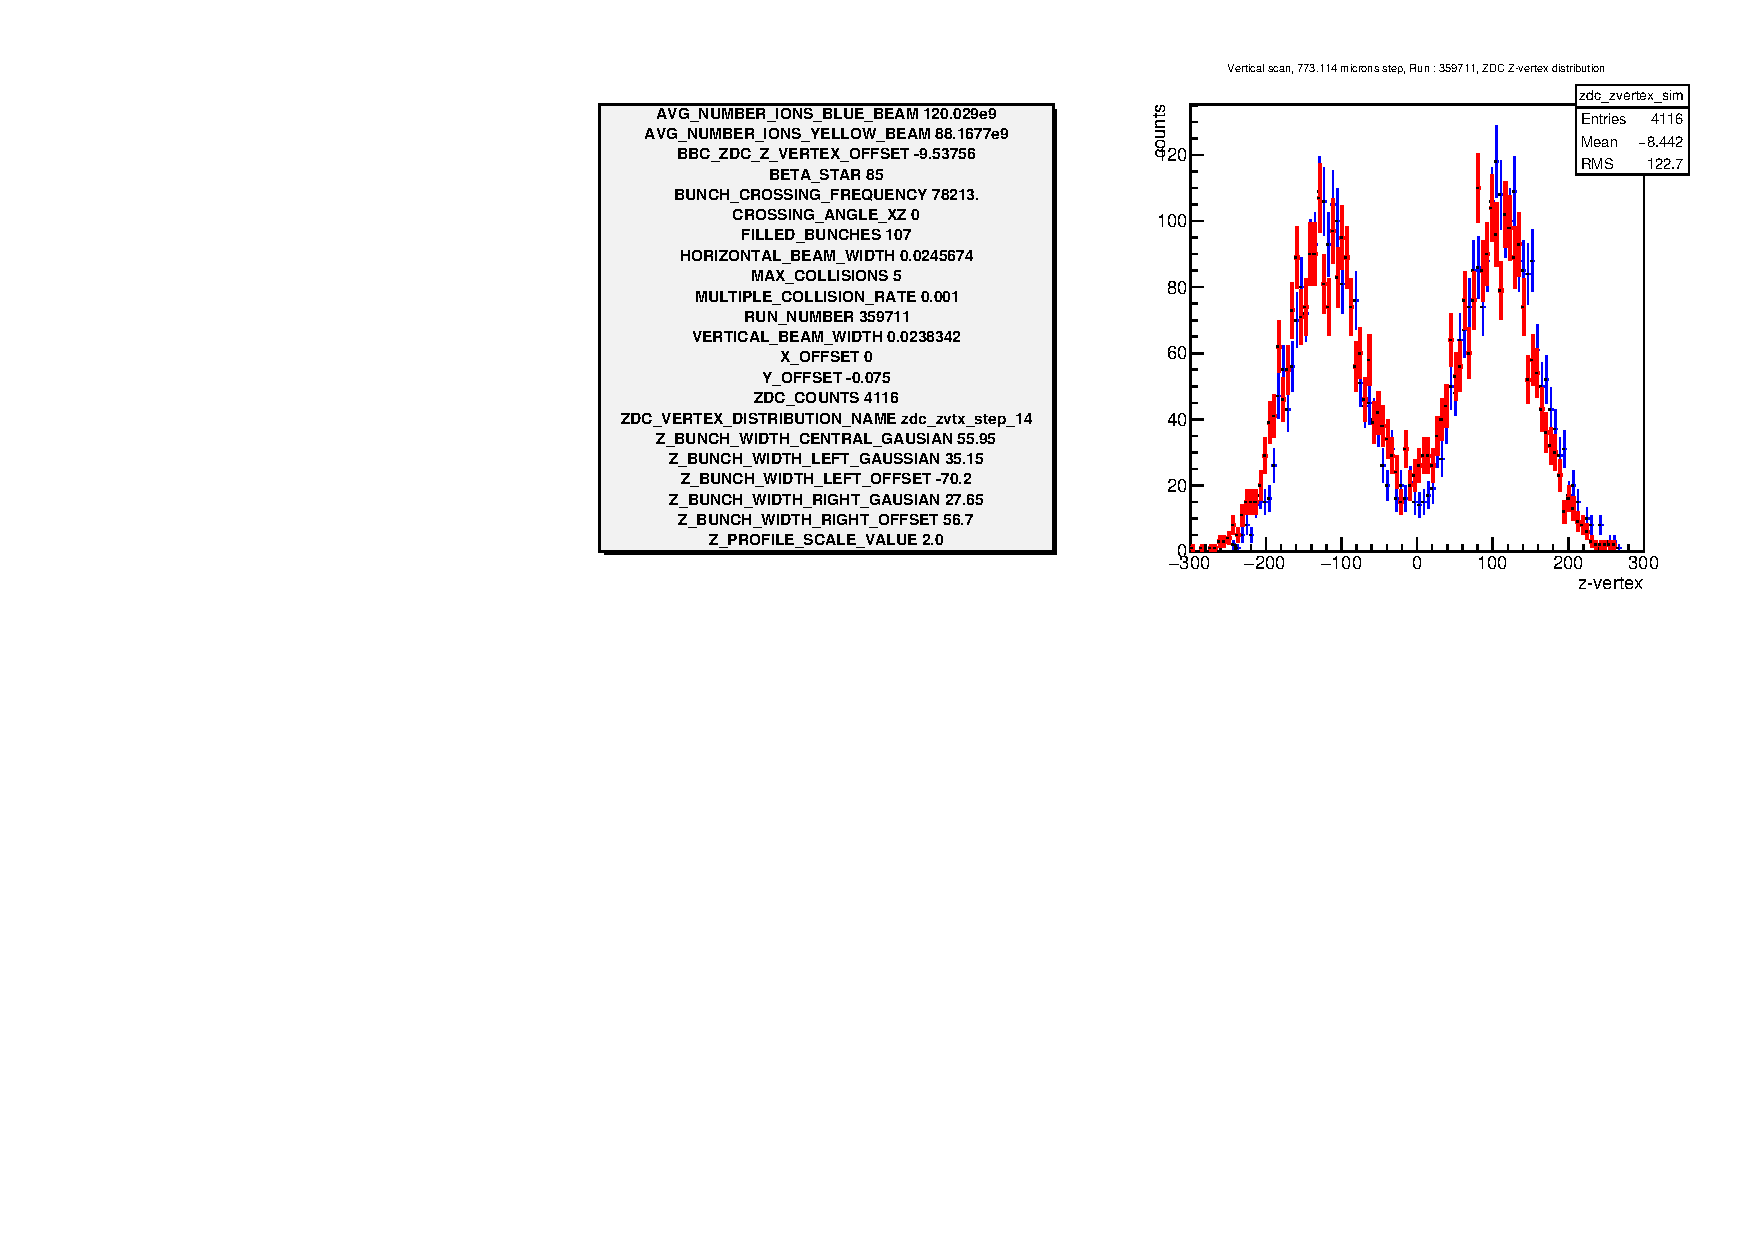
\includegraphics[width=\linewidth,height=\textheight,keepaspectratio]{./figures/359711_step14_config_compare}
\caption{ 
\textcolor{red}{Default Caption}
}
\label{fig:359711_step14_config_compare}
\end{center}
\end{figure}
\clearpage

By running the simulation with extreme variations in the parameters,
systematically, I identified how each parameter tends to affect the z-vertex
profile. The following parameters map to the following z-profile behavior:
\begin{itemize}
  \item $\theta_{XZ} \rightarrow$ Asymmetry in peak heights
  \item Beam Displacement / $\sigma{x,y} \rightarrow$ Peak Separation
  \item ZDC yield (not shown) $\rightarrow$ Peak Scaling
\end{itemize}

Also note that scaling the beam widths OR changing the displacement will change
the total amount of overlapping beam. It was also determined that we cannot
observe the effects of vertical-beam width scaling or YZ crossing angle during a
horizontal beam displacement, similarly in the horizontal case.

Detailed slides on this study were presented to the Spin PWG on 11 November
2015, the slides are attached to the Agenda under speaker "Mike Beaumier".
